\documentclass{article}
\usepackage{graphicx}
\graphicspath{ {./images/} }
\usepackage[export]{adjustbox}
\usepackage{amsmath}


\title{12. Polinomu LKD un saknes.}
\author{Gunārs Ābeltiņš}
\date{2022-05-20}

\begin{document}

\maketitle

\section*{1. Uzdevums}
1. Parādot visus aprēķina soļus, atrodiet lielāko kopīgo dalītāju šādam polinomu pārim: 2x5-5x4+6x3+3x2-2x+8, 2x5-7x4+12x3-8x2+7x-4. Rezultātu pārbaudiet ar WolframAlpha.

\begin{equation*}
    P(x) = 2x^5-5x^4+6x^3+3x^2-2x+8
\end{equation*}
\begin{equation*}
    Q(x) = 2x^5-7x^4+12x^3-8x^2+7x-4
\end{equation*}
\begin{gather*}
    LKD(P(x), Q(x)) \\
    P_1 = P - Q = \\ = (2x^5-5x^4+6x^3+3x^2-2x+8) - (2x^5-7x^4+12x^3-8x^2+7x-4) = \\ = 2x^4-6x^3+11x^2-9x+12
\end{gather*}
\begin{gather*}
    LKD(2x^4-6x^3+11x^2-9x+12, 2x^5-7x^4+12x^3-8x^2+7x-4) \\
    Q_1 = Q - xP_1 = \\ = (2x^5-7x^4+12x^3-8x^2+7x-4) - x(2x^4-6x^3+11x^2-9x+12) = \\ = -x^4+x^3+x^2-5x-4
\end{gather*}
\begin{gather*}
    LKD(2x^4-6x^3+11x^2-9x+12, -x^4+x^3+x^2-5x-4) \\
    P_2 = P_1 + 2Q_1 = \\ = (2x^4-6x^3+11x^2-9x+12) + 2(-x^4+x^3+x^2-5x-4) = \\ = -4x^3+13x^2-19x+4
\end{gather*}
\begin{gather*}
    LKD(-4x^3+13x^2-19x+4, -x^4+x^3+x^2-5x-4) \\
    Q_2 = 4Q_1 - xP_2 = \\ = 4(-x^4+x^3+x^2-5x-4) - x(-4x^3+13x^2-19x+4) = \\ = -9x^3+23x^2-24x-16
\end{gather*}
\begin{gather*}
    LKD(-4x^3+13x^2-19x+4, -9x^3+23x^2-24x-16) \\
    P_3 = 9P_2 - 4Q_2 = \\ = 9(-4x^3+13x^2-19x+4) - 4(-9x^3+23x^2-24x-16) = \\ = 25x^2-75x+100
\end{gather*}
\begin{gather*}
    LKD(25x^2-75x+100, -9x^3+23x^2-24x-16) \\
    Q_3 = Q_2 + \frac{9}{25}xP_3 = \\ = (-9x^3+23x^2-24x-16) + \frac{9}{25}x(25x^2-75x+100) = \\ = -4x^2+12x-16
\end{gather*}
\begin{gather*}
    LKD(25x^2-75x+100, -4x^2+12x-16) \\
    P_4 = \frac{1}{25}P_3 + \frac{1}{4}Q_3 = \\ = \frac{1}{25}(25x^2-75x+100) + \frac{1}{4}(-4x^2+12x-16) = \\ = 0
\end{gather*}
\begin{equation*}
    \frac{25x^2-75x+100}{25} = x^2-3x+4
\end{equation*}
\begin{equation*}
    LKD(P(x), Q(x)) = x^2-3x+4
\end{equation*}
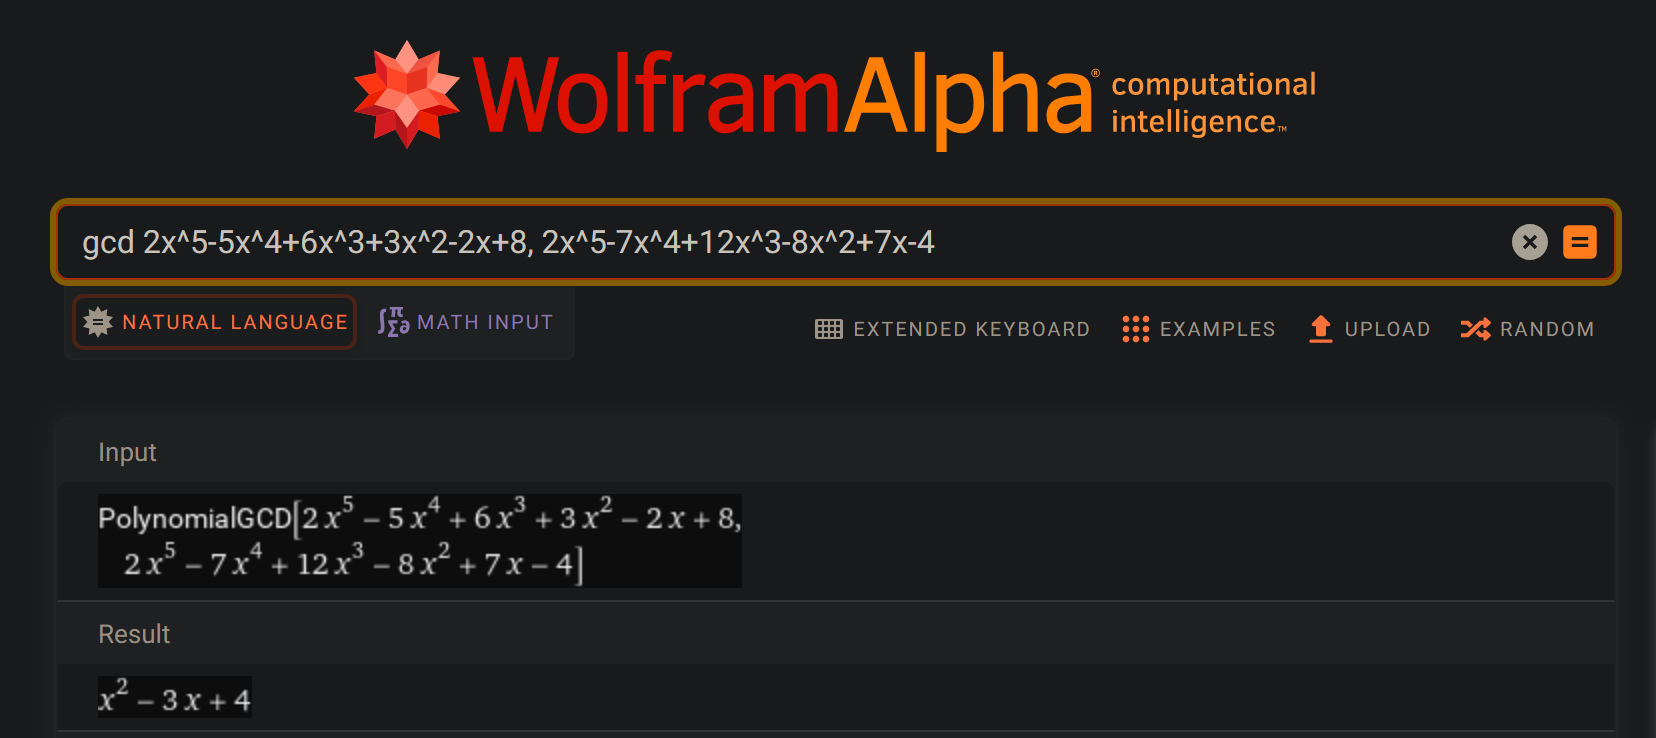
\includegraphics[width=0.9\textwidth, center]{1.png}

\section*{2. Uzdevums}
a) Uzrakstiet kanoniskajā pierakstā divus 3.pakāpes polinomus: P, kura saknes ir 1, 2 un 5; Q, kura saknes ir 2, 3 un 5.  Atrodiet LKD(P, Q).

\begin{equation*}
    P(x) = (x-1)(x-2)(x-5)
\end{equation*}
\begin{equation*}
    Q(x) = (x-2)(x-3)(x-5)
\end{equation*}
\begin{equation*}
    LKD(P(x), Q(x)) = (x-2)(x-5)LKD(x-1, x-3) = (x-2)(x-5)
\end{equation*}

b) (LABOTS 11.05 19:40) Uzrakstiet divus 4.pakāpes polinomus, kuriem visas saknes ir reālas un kuru LKD ir 2x2-3. Rezultātus pārbaudiet ar WolframAlpha.

\begin{equation*}
    P(x) = (2x^2-3)(x-1)(x-2)
\end{equation*}
\begin{equation*}
    Q(x) = (2x^2-3)(x-3)(x-4)
\end{equation*}
\begin{equation*}
    LKD(P(x), Q(x)) = (2x^2-3)
\end{equation*}
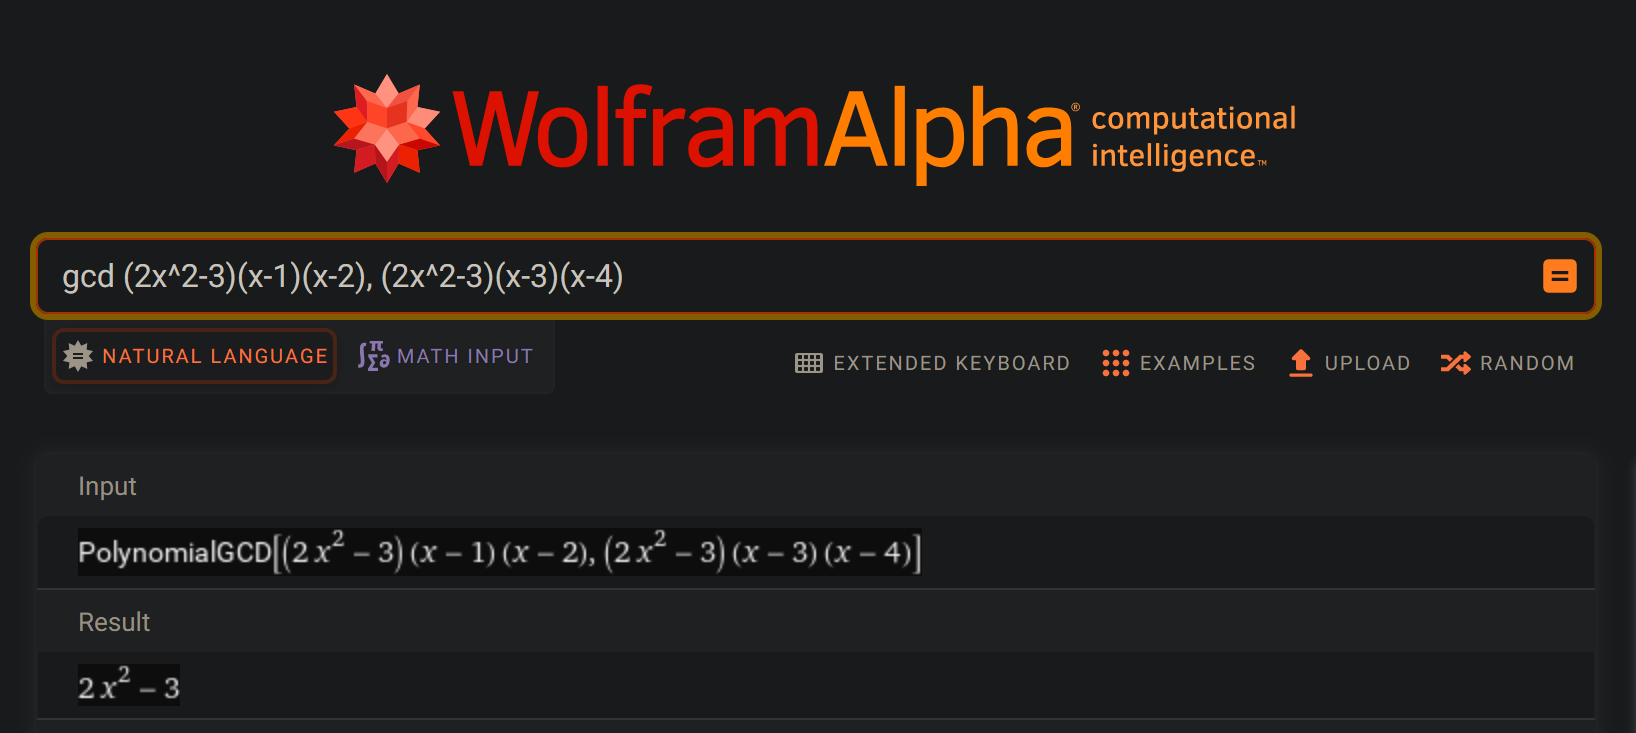
\includegraphics[width=0.9\textwidth, center]{2}

\section*{3. Uzdevums}
Izmantojot WolframAlpha vai citu līdzekli, sadaliet lineāros reizinātājos slaveno polinomu x5-x+1. Saknes ņemiet ar precizitāti 0,01.

\begin{gather*}
    x^5-x+1 = \\ = (x-1.17)(x-(0.76 - 0.35i))(x-(-0.18 + 1.08i))\\(x-(-0.18 - 1.08i))(x-(0.76 + 0.35i))
\end{gather*}

\end{document}